\title{%
  Accountability
}
\author{Daniel Bosk}
\institute[MIUN IKS]{%
  Department of Information and Communication Systems,\\
  Mid Sweden University, SE-851\,70 Sundsvall.
}
\date{\today}


\begin{frame}
  \titlepage{}
\end{frame}

\begin{frame}
  \tableofcontents
\end{frame}


% Since this a solution template for a generic talk, very little can
% be said about how it should be structured. However, the talk length
% of between 15min and 45min and the theme suggest that you stick to
% the following rules:  

% - Exactly two or three sections (other than the summary).
% - At *most* three subsections per section.
% - Talk about 30s to 2min per frame. So there should be between about
%   15 and 30 frames, all told.


\section{Book-Keeping}

\subsection{Double-Entry Book-Keeping}

\begin{frame}
  \begin{itemize}
    \item The banks are one of the oldest institutions with a need for strict 
      accountability.

    \item The main tools developed for this purpose is double-entry 
      book-keeping.
  \end{itemize}
\end{frame}

\begin{frame}
  \begin{definition}[Double-entry book-keeping]
    \begin{itemize}
      \item Add one entry of \(x\) and one of \(-x\).
      \item Invariant of zero (\(x+(-x) = 0\)).
    \end{itemize}
  \end{definition}

  \begin{example}
    \begin{itemize}
      \item All books should be balanced.

      \item A transfer from one account to another must be a credit in one 
        account and a debit in the other.

      \item I.e.\ when adding them up they equal zero.
    \end{itemize}
  \end{example}
\end{frame}

\begin{frame}
  \begin{itemize}
    \item This principle of keeping a balance of constant zero can be 
      tranferred to other principles.

    \item E.g.\ for each log-in there should be a log-out.

    \item If the difference of number of log-ins \(L_i\) for a user and the 
      number of log-outs \(L_o\) is zero (\(L_i-L_o = 0\)), then the user is 
      not currently logged-in.

    \item Hence, the user shouldn't be able to post a comment when the system 
      is in this state.
  \end{itemize}
\end{frame}

\begin{frame}
  \begin{remark}
    \begin{itemize}
      \item Note that you shouldn't use the book-keeping system to keep track of 
        whether a user is logged-in or not.

      \item You can use more efficient mechanisms for that.

      \item But the account should be kept for future reference, in case 
        something bad happens, then you should be able to see what really 
        happened.
    \end{itemize}
  \end{remark}
\end{frame}

\subsection{Separation of Duties}

\begin{frame}
  \begin{definition}[Separation of duties]
    \begin{itemize}
      \item Two or more entities must collude to break the policy.
      \item Two classes: \emph{dual control} and \emph{functional separation}.
    \end{itemize}
  \end{definition}
\end{frame}

\begin{frame}
  \begin{example}[Dual control]
    \begin{itemize}
      \item Two or more staff members must act together to authorize 
        a transaction.
    \end{itemize}
  \end{example}

  \pause{}

  \begin{example}[Dual control on film]
    \begin{itemize}
      \item Two guys in a nuclear weapons silo.
      \item Two keys too far from each other for one to turn simultaneously.
      \item Both staffers must agree to turn the keys.
    \end{itemize}
  \end{example}
\end{frame}

\begin{frame}
  \begin{example}[Functional separation]
    \begin{itemize}
      \item Two or more staff members must act on the transaction at different 
        points in the transaction path.
    \end{itemize}
  \end{example}
  
  \pause{}

  \begin{example}[Functional separation]
    \begin{itemize}
      \item Developer team writes the code.
      \item System administrators deploy it.
      \item Auditors verifies security.
    \end{itemize}
  \end{example}
\end{frame}

\subsection{Clark-Wilson Security Policy Model}

\begin{frame}
  \begin{itemize}
    \item The Clark-Wilson Security Policy Model is a model for securely 
      implementing a security policy.

    \item It ensures \emph{internal consistency}, i.e.\ properties of the 
      internal state of the system.

    \item It also allows for \emph{external consistency}, i.e.\ the relation of 
      the internal state of the system to the real world.
      This must however be enforced by e.g.\ auditing.
  \end{itemize}
\end{frame}

\begin{frame}
  \begin{itemize}
    \item Mechanisms for enforcing integrity of the system are:
      \begin{itemize}
        \item Well-formed transactions

        \item Separation of duties
      \end{itemize}
  \end{itemize}

  \pause{}

  \begin{definition}[Well-formed transactions]
    \begin{itemize}
      \item A limited set of functions can manipulate an object.
      \item Users have access to these functions, not the objects.
    \end{itemize}
  \end{definition}
\end{frame}

\begin{frame}
  \begin{block}{Requirements}
    \begin{enumerate}
      \item Subjects have to be identified and authenticated.
      \item Objects can be manipulated only by a restricted set of functions.
      \item Subjects can execute only a restricted set of functions.
      \item A proper audit log must be maintained.
      \item The system has to be certified to work properly.
    \end{enumerate}
  \end{block}
\end{frame}

\begin{frame}
  \begin{definition}[Unconstrained data item, UDI]
    \begin{itemize}
      \item Input from outside the system.
      \item From outside the control of the system.
      \item It can be anything!
    \end{itemize}
  \end{definition}

  \pause{}

  \begin{definition}[Constrained data item, CDI]
    \begin{itemize}
      \item Objects (data) inside the system.
      \item This is under the system's control.
      \item This is well-formed.
    \end{itemize}
  \end{definition}
\end{frame}

\begin{frame}
  \begin{remark}
    \begin{itemize}
      \item UDIs must be converted to CDIs.
      \item This is a critical part of the system.
    \end{itemize}
  \end{remark}
\end{frame}

\begin{frame}
  \begin{definition}[Transformation procedure, TP]
    \begin{itemize}
      \item Procedure which manipulates CDIs.
      \item Can take UDI as input, must convert to CDI.
    \end{itemize}
  \end{definition}

  \pause{}

  \begin{definition}[Integrity verification procedure, IVP]
    \begin{itemize}
      \item Checks the integrity of a CDI.
    \end{itemize}
  \end{definition}
\end{frame}

\begin{frame}
  \begin{block}{Certification rules}
    Should be checked so that the policy is consistent:
    \begin{description}
      \item[CR1] IVPs must ensure integrity of CDIs when IVPs are run.
      \item[CR2] TPs must be certified to be valid; valid CDIs transform into 
        valid CDIs; each TP can access restricted set of CDIs.
      \item[CR3] Access rules must satisfy separation-of-duties requirements.
      \item[CR4] All TPs must write to an append-only log.
      \item[CR5] Any TP handling UDI must convert it to a CDI or reject it.
    \end{description}
  \end{block}
\end{frame}

\begin{frame}
  \begin{block}{Enforcement rules}
    Describes the mechanisms needed in the system:
    \begin{description}
      \item[ER1] Must maintain and protect list of CDIs each TP can access.
      \item[ER2] Must maintain and protect list of TPs each subject can access.
      \item[ER3] The system must authenticate each subject requesting to execute 
        a TP\@.
      \item[ER4] Only a subject that may certify an access rule for a TP may 
        modify the respective entry in the list.
        This subject must not be allowed to execute this TP\@.
    \end{description}
  \end{block}
\end{frame}


\section{Logging}

\subsection{Securing Logging Mechanisms}

\begin{frame}
  \begin{itemize}
    \item Have a process write log messages to a file.

    \item Then the running process must access the file.
      \begin{itemize}
        \item Could be done using append only access, thus no reading or 
          rewriting.

        \item Could trust the process to do a setuid(2) system call.

        \item This saves us from trusting the user -- but only if the user 
          doesn't have access to the hardware.

      \end{itemize}

    \item We could also log to this or another system via syslog(3), this helps 
      us if we don't trust the user or the process.

    \item However, the problem remains with the sysadmin who has superuser 
      access to the system.

  \end{itemize}
\end{frame}

\begin{frame}
  \begin{itemize}
    \item The sysadmin problem can be solved using a clever setup of separation 
      of duty.

    \item E.g.\ the logs of sysadmin \(A\) will be stored under the control of 
      sysadmins \(B\) and \(C\).

    \item This way sysadmin \(A\) can do everything except modify his own 
      logging mechanisms.

    \item The downside of this is that all systems must be online for this to 
      work.

  \end{itemize}
\end{frame}

\subsection{Schneier-Kelsey Logs}

\begin{frame}
  \begin{itemize}
    \item The Schneier-Kelsey logging scheme provides a secure logging 
      mechanism for storing logs in an untrusted machine.

    \item The untrusted machine \(\U\) is expected to work correctly up to 
      a time \(t\) when it is compromised by an attacker.

    \item The logging mechanism and the integrity of the logs \(L_1, \ldots, 
      L_{t-1}\) before \(t\) are provided with confidentiality and integrity.

    \item All logs \(L_t, L_{t+1}, \ldots\) generated from this point, however, 
      are under the influence of the attacker.

  \end{itemize}
\end{frame}

\begin{frame}
  \begin{itemize}
    \item The scheme consists of an untrusted principal \(\U\) and a trusted 
      principal \(T\).

  \end{itemize}
\end{frame}

\begin{frame}
  \begin{figure}
    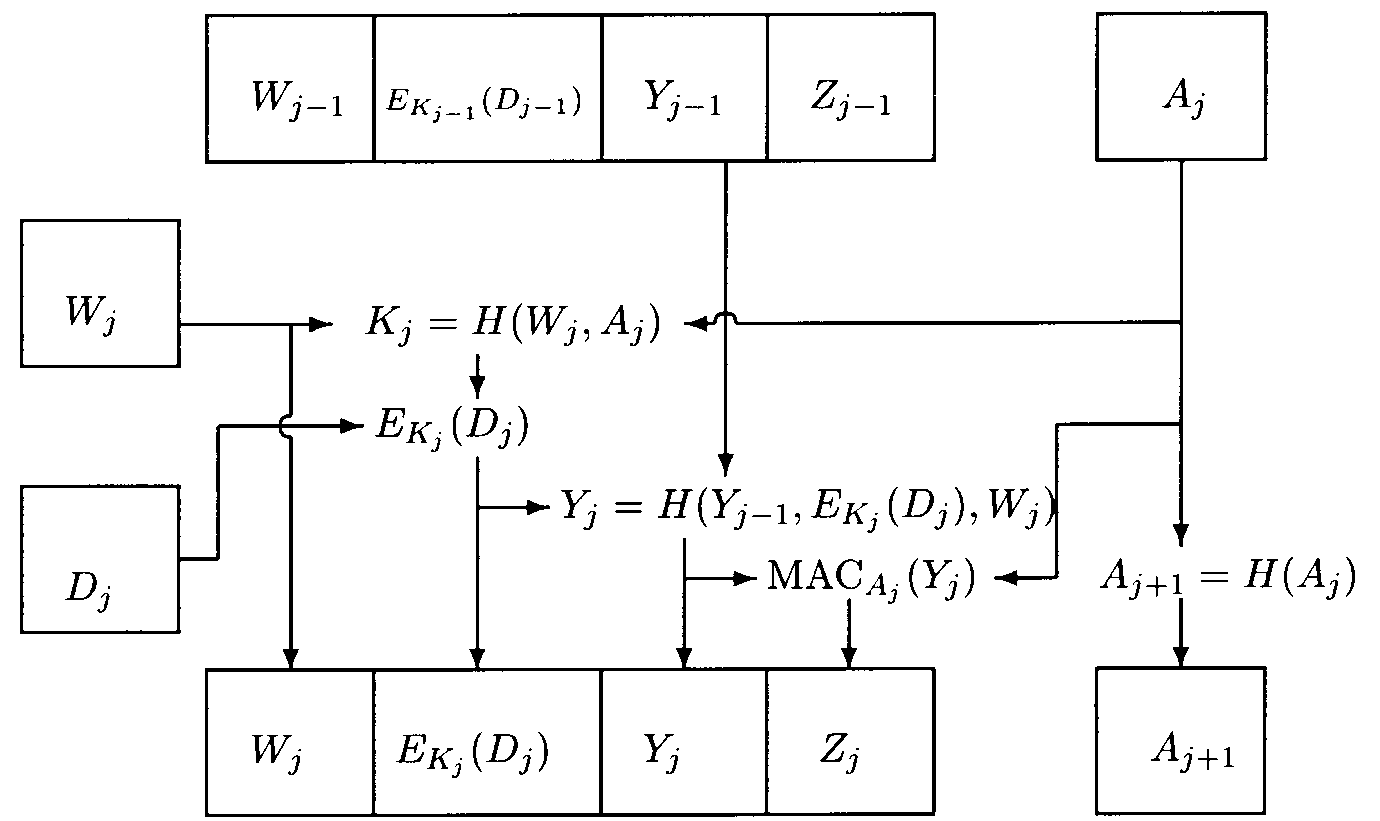
\includegraphics[height=0.7\textheight]{seclog.png}
    \caption{%
      Overview of Schneier-Kelsey secure-log scheme; where \(W_j\) is the type 
      of entry, \(D_j\) is entry data, \(K_j\) is entry key, \(A_j\) is 
      authentication key, and \(H\) is a one-way function.
      Image:~\cite{schneier1999secure}.
    }
  \end{figure}
\end{frame}

\begin{frame}
  \begin{itemize}
    \item One interesting property is that validation of logs can be delegated 
      to a third party verifier \(\V\).
  \end{itemize}
\end{frame}


%%%%%%%%%%%%%%%%%%%%%%

\begin{frame}
  \small
  \printbibliography{}
\end{frame}

